\documentclass[14pt, a4paper]{report}
\usepackage{mathtext}
\usepackage[T2A]{fontenc}
\usepackage[utf8]{inputenc}
\usepackage[russian]{babel}
\usepackage{multirow}
\usepackage{graphicx}
\renewcommand{\thesection}{\arabic{section}.}

\title{\textbf{Отчет о выполнении лабораторной работы 2.2.1 "Исследование взаимной диффузии газов"}}
\author{Калашников Михаил, Б03-205}
\date{}

\begin{document}
\maketitle

\textbf{Цель работы:}
регистрация зависимости концентрации гелия в воздухе от времени с помощью датчиков теплопроводности при разных начальных давлениях смеси газов; определение коэффициента диффузии по результатам измерений.
\newline

\textbf{В работе используются:}
\begin{itemize}
\item измерительная установка ($V_1=V_2=800\pm5\ см^3,\ l/S=15,0\pm0,1\ \frac{1}{см}$);
\item форвакуумный насос;
\item баллон с газом (гелий);
\item манометр ($\sigma_P=0,005\cdot 760\ торр=3,8\ торр$);
\item источник питания;
\item магазин сопротивлений;
\item гальванометр;
\item секундоменр;
\end{itemize}

\section{Теоретическая часть}

Диффузией называется самопроизвольное перемешивание молекул, происходящее вследствие их теплового движения.
Плотность диффузионного потока любого компонента (т. е. количество вещества, проходящее в единицу времени через единичную поверхность) определяется законом Фика:
\[j=-D\frac{\partial n}{\partial x}\]
где $D$ -- коэффициент взаимной диффузии газов, а $j$ -- плотность потока частиц.
Применяя этот закон к условиям нашего эксперимента совместно с законом сохранения вещества, можно получить уравнение, описывающее изменении разности концетраций от времени.
\[n_1-n_2=(n_1-n_2)_0e^{-t/\tau},\quad\tau=\frac{V_1V_2}{V_1+V_2}\frac{l}{SD}\]

\section{Экспериментальная установка}

\begin{figure}[!ht]
\centering
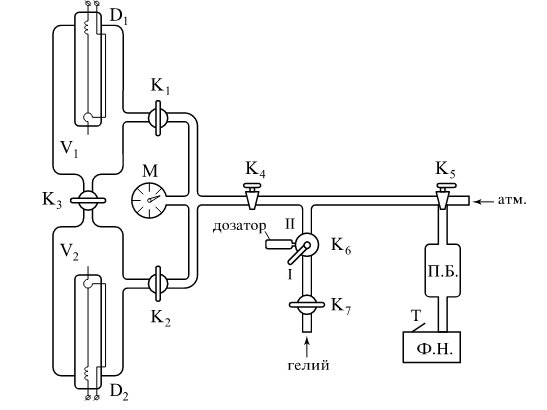
\includegraphics[width=0.6\linewidth]{terma_4_1.png}
\caption{Установка для исследования взаимной диффузии газов}
\end{figure}

Для исследования взаимной диффузии газов и определения коэффициента диффузии используется установка, изображенная на рис. 1. Два сосуда с объемами V1 и V2 соединены трубкой длины l и сечения S. Сосуды заполнены смесью двух газов при одинаковом давлении, но с различной концентрацией компонентов. Вследствие взаимной диффузии концентрации каждого из компонентов в обоих сосудах с течением времени выравниваются.

\begin{figure}[!ht]
\centering
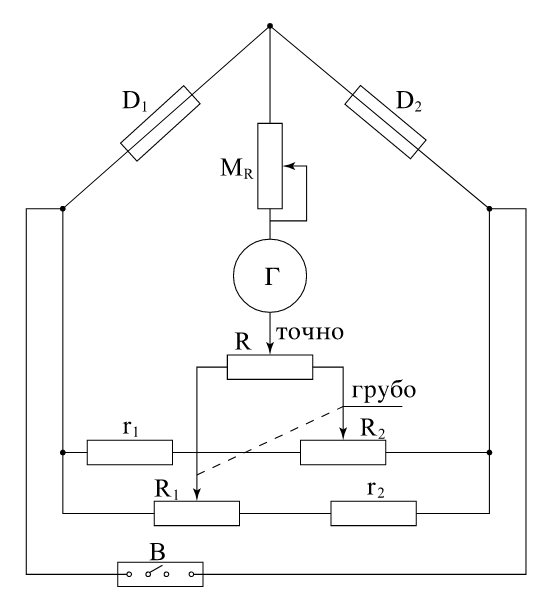
\includegraphics[width=0.6\linewidth]{terma_4_2.png}
\caption{Мостовая схема с датчиками теплопроводности для измерения разности концентраций газов}
\end{figure}

Для измерения концентраций в данной установке применяются датчики теплопроводности $D_1$, $D_2$ и используется зависимость теплопроводности газовой смеси от ее состава. Тонкая проволочка радиуса $r_{pr}$, протянутая вдоль оси стеклянного цилиндра радиуса $R_{c}$, нагревается током. Тепло от проволочки к стенке цилиндра переходит главным образом вследствие теплопроводности газа, находящегося внутри цилиндра.

\section{Проведение эксперимента}

\begin{enumerate}

\item Ознакомимся с установкой. Изучим действие каждого из присутствующих на установке кранов, инструкцию работы с форвакуумным насосом.

\item Установка включена в сеть, октроем краны К1 - К3.

\item С помощью форвакуумного насоса откачаем воздух из установки. Выключим насос, не забыв соединить его с атмосферой.

\item Напустим в установку воздух до рабочего давления $P$. В начале эксперимента оно равно 40 торр. Сбалансируем мост, перекрыв краны К1 и К2.

\item Заполним верхнюю емкость гелием до давления, равного $0.2P$. Для этого откроем кран К7 и возпользуемся дозатором К6. Закрыв кран К1 и откачав гелий, оставшийся в патрубках, заполним нижнюю емкость воздухом из атмосферы до давления $1.75P$ с помощью крана К5. Далее дадим давления в обоих емкостях уравняться, открыв для этого краны К1 и К2 на ~30 секунд. Запишем установившееся давление. 

\item Приступим к измерениям. Откроем кран К3 и сразу после этого запустим компьютерную программу. Будем продолжать процесс измерения, пока показания вольтметра не опустятся на 30-50\%. Сохраним полученные измерения, указав установившееся давление.

\item Поднимем рабочее давление на 40 торр и повторим три последних пункта. Будем продолжать это вплоть до давления в 240 торр.

\end{enumerate}

\section{Обработка данных}

\begin{enumerate}

\setcounter{enumi}{7}

\item Автоматизированные измерения позволили снять примерно 4000 точек за все время эксперимента, поэтому приводить их в отчете в виде таблицы не имеет смысла. По этим точкам мы построим зависимость $\ln V(t)$. В таблицу 1 внесем угловые коэффициенты полученных прямых $k$ и вычисленные на основании последних коэффициенты взаимной диффузии $D$ по формуле:
\[\ln P=-\frac{t}{\tau}+\ln P_0=kt+\ln P_0\]
\[D=\frac{1}{\tau}\frac{V_1V_2}{V_1+V_2}\frac{l}{S}=-k\frac{V_1V_2}{V_1+V_2}\frac{l}{S}\]

\item Построим график зависимости $D(1/P)$. Продлим прямую до точки $(1/P_0; D_0)$, где $P_0$ -- атмосферное давление, $D_0$ -- коэффициент взаимной диффузии при атмосферном давлении.

\item Вычисли длину свободного пробега $\lambda$ и размер молекулы $r$. Для этого воспользуемся формулами:
\[D_0=\frac{1}{3}\lambda\langle v\rangle,\quad \langle v\rangle=\sqrt{\frac{8RT}{\pi\mu}}\]
\[\lambda=\frac{3D_0}{\langle v\rangle}=3D_0\sqrt{\frac{\pi\mu}{8RT}}\]
\[\pi(2r)^2\lambda n=1,\quad n=\frac{P_0}{kT}\]
\[r=\frac{1}{2\sqrt{\pi\lambda n}}=\frac{1}{2}\sqrt{\frac{kT}{\pi\lambda P_0}}\]
где $k$ -- постоянная Больцмана, $P_0$ -- атмосферное давление, $T=297\pm2\ К$, $\mu$ -- молярная масса гелия.

\end{enumerate}

\section{Расчет погрешностей}
Найдем среднюю погрешность значения коэффициента взаимной диффузии:
\[\varepsilon_{D,\ приб}=\sqrt{\varepsilon_V^2+\varepsilon_{\frac{l}{S}}^2}=0,9\%,\ т.к.\ V_1=V_2=V\ и\  \sigma_{V_1}=\sigma_{V_2}\]
\[\varepsilon_{D,\ случ}=\langle\varepsilon_k\rangle=\langle\frac{\sigma_k}{k}\rangle=0,1\%\]
\[\varepsilon_{D}=\sqrt{\varepsilon_{D,\ приб}^2+\varepsilon_{D,\ случ}^2}=0,9\%\]

Отсюда найдем погрешность $D_0$:
\[D_0\approx D\frac{P}{P_0},\quad\varepsilon_{D_0}=\sqrt{\varepsilon_D^2+\varepsilon_P^2}=4,0\%\]
\[где\ \varepsilon_P=\sigma_P\langle\frac{1}{P}\rangle=3,9\%\]

Таким образом:
\[D_0=0,81\pm0,03\ \frac{{см}^2}{с}\]

Воспользуемся формулой погрешности косвенных измерения для определения погрешности $\lambda$ и $r$.
\[\varepsilon_\lambda=\sqrt{\varepsilon_{D_0}^2+\frac{1}{4}\varepsilon_T^2}=4,0\%\]
\[\lambda=195\pm8\ нм\]
\[\varepsilon_r=\frac{1}{2}\sqrt{\varepsilon_{\lambda}^2+\varepsilon_T^2}=2,0\%\]
\[r=129\pm3\ пм\]

\section{Вывод}

Полученные величины сходятся с значениями, приводимых в справочниках. Это свидетельствует корректности и точности проведенного эксперимента. 

\section{Приложения}
\begin{table}[!ht]
\centering
\makebox[\textwidth][c] {
\begin{tabular}{| c | c | c | c | c | c | c |}
\hline
$P,\ торр$ & 40 & 80 & 120 & 160 & 200 & 240 \\
\hline
$k,\ 10^{-3}/с$ & -2,136 & -1,005 & -0,747 & -0,553 & -0,446 & -0,386 \\
\hline
$D,\ см^2/с$ & 12,82 & 6,03 & 4,48 & 3,32 & 2,68 & 2,32 \\
\hline
\end{tabular}
}
\label{table1}
\caption{Вычисления коэффициента взаимной диффузии при различных давлениях}
\end{table}

\begin{figure}[!ht]
\centering
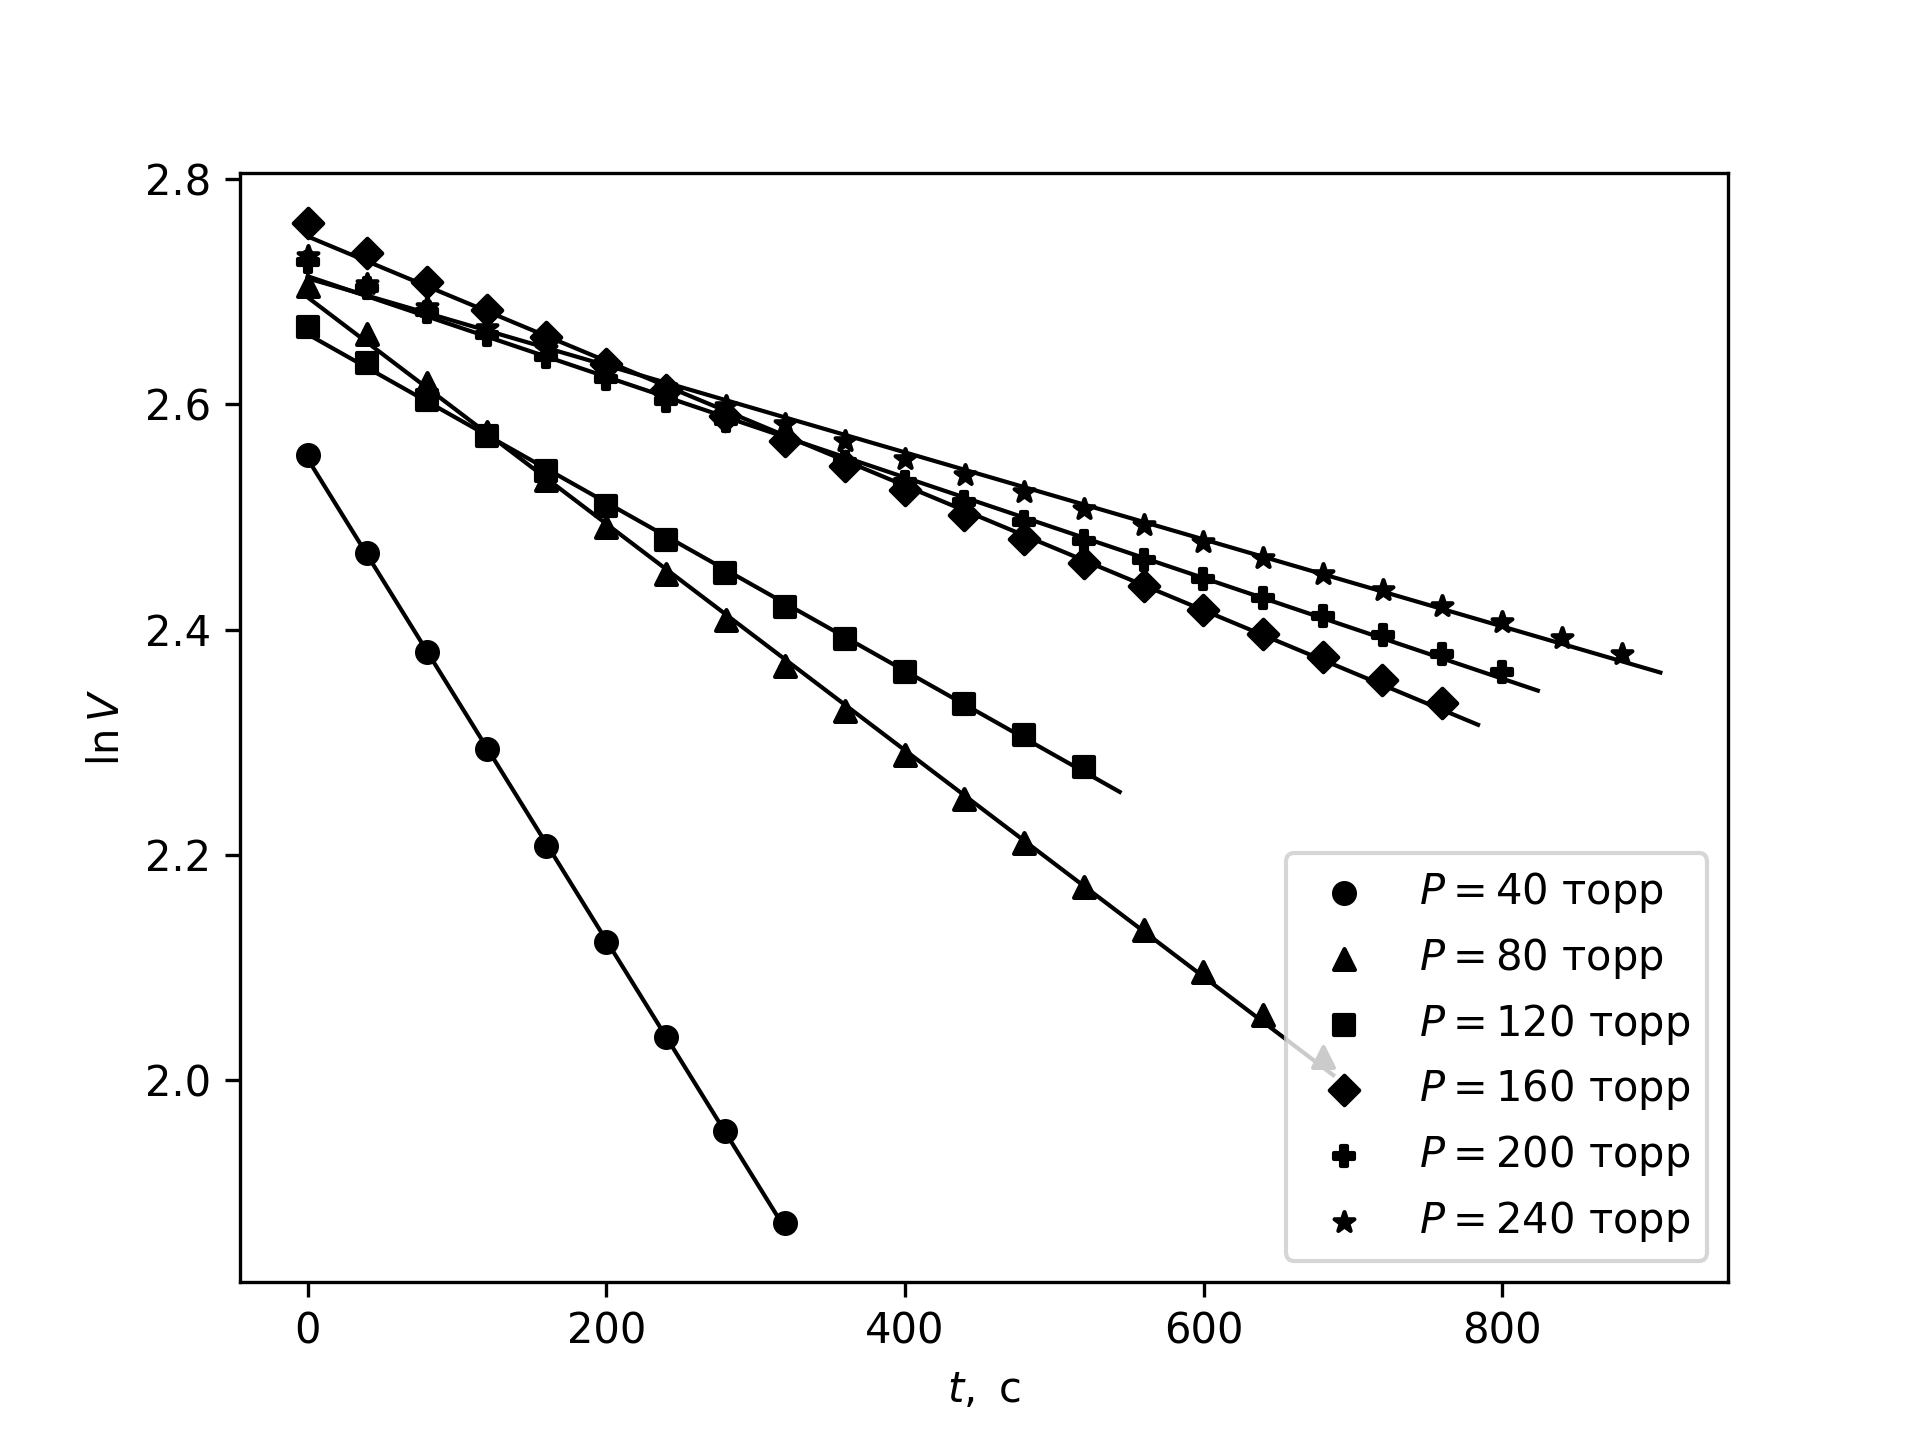
\includegraphics[scale=0.8]{terma_4_3.png}
\caption{График зависимости $\ln V(t)$}
\end{figure}

\begin{figure}[!ht]
\centering
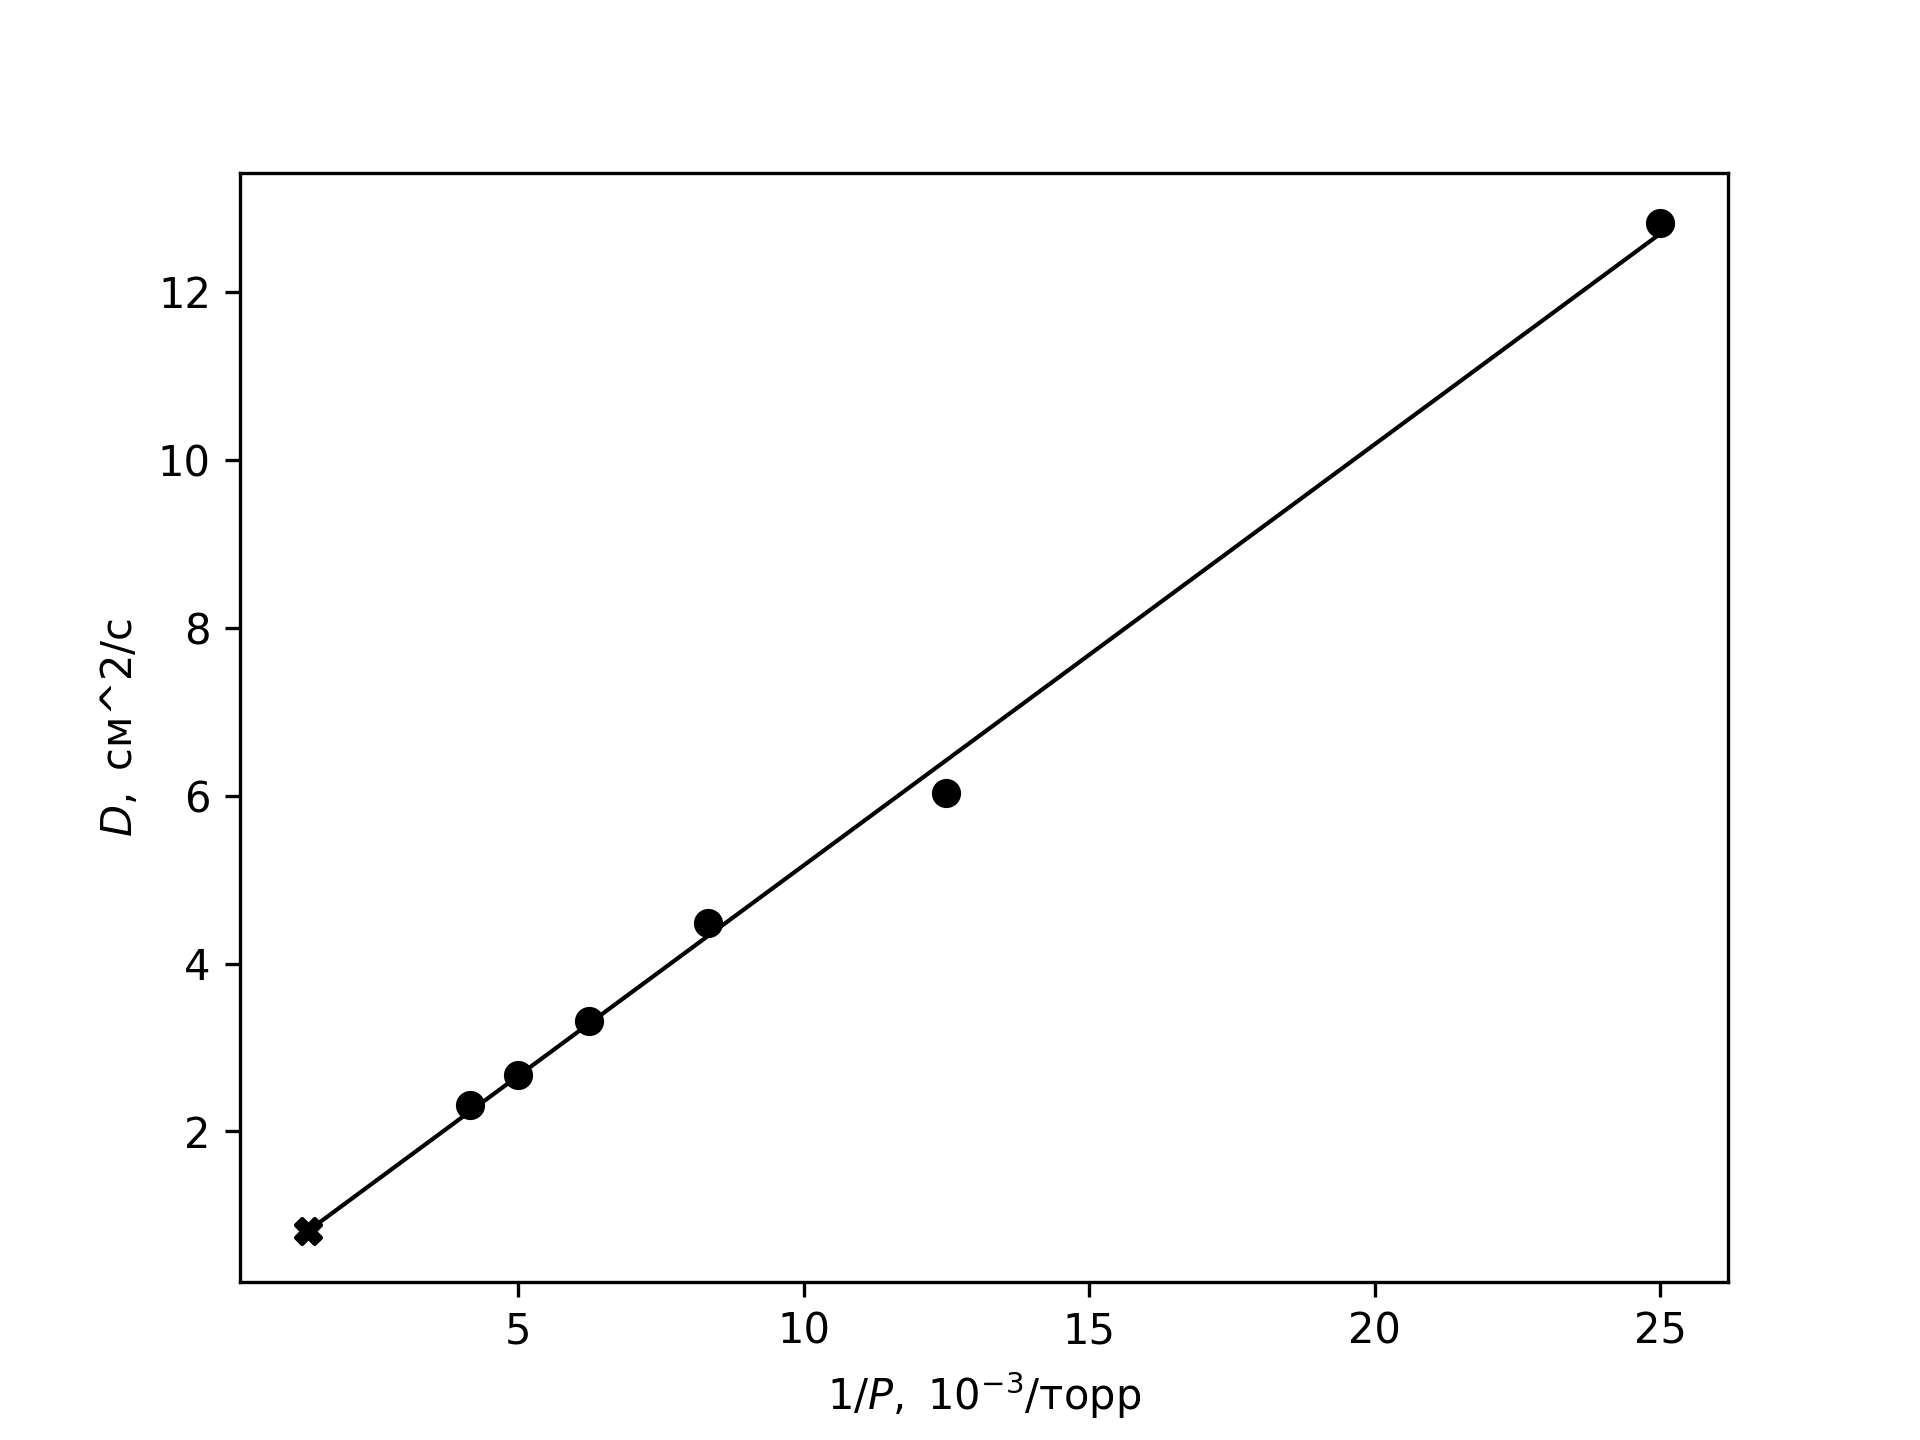
\includegraphics[scale=0.8]{terma_4_4.png}
\caption{График зависимости $D(1/P)$}
\end{figure}


\end{document}